% 第 27 题前灯抛物面反射镜轴截面图：源为嵌入位图（938×1392），按题设数据等比作图实测
% （1 cm = 5.77 pt；页面坐标 y 向下换算 Y = 490 − y_page）。
% 照源要点：抛物线 y² = 14.4x 精确作图（灯口半径 12 cm 处与椭圆上下端点重合）；
% 灯口圆面画为透视椭圆（纵半轴 = 12 cm，横半轴 14.3 pt，轴比 0.203）；
% 椭圆内竖虚线自中心向下至椭圆下端附近（源内上半段未画）；24cm 竖排标注、10cm 横排标注
% （尺寸线在文字处断开），尺寸线两端向外实心箭头，Times 正体「cm」。
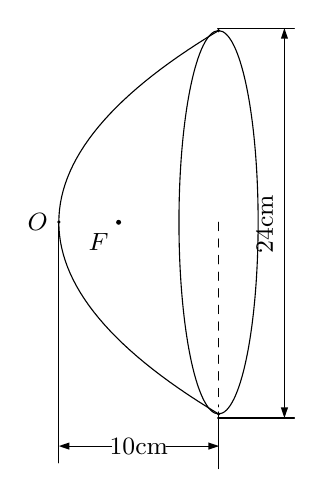
\begin{tikzpicture}[line cap=round,line join=round,font=\small,x=0.03515cm,y=0.03515cm]
% ===== 抛物线（y² = 14.4 x，ξ 以 cm 计，ξ ∈ [−12,12]）=====
\draw plot[domain=-12:12,samples=61,variable=\t] ({441.1+5.77*(\t*\t/14.4)}, {91.6+5.77*\t});
% ===== 灯口透视椭圆（与抛物线两端点重合）=====
\draw (498.8,91.6) ellipse [x radius=14.3, y radius=69.24];
% ===== 椭圆内竖直虚线（自中心向下，照源上半段未画）=====
\draw[dashed] (498.8,91.6)--(498.8,24.9);
% ===== 焦点 F（实心点）与 O 顶点、抛物线-椭圆上下接合处小点（照源）=====
\fill (462.7,91.6) circle[radius=0.9pt];
\fill (441.1,91.7) circle[radius=0.65pt];
\fill (498.8,160.84) circle[radius=0.65pt];
\fill (498.8,22.36) circle[radius=0.65pt];
% ===== 24cm 尺寸线（竖直，两端向外箭头）与上下水平引出线 =====
\draw (498.5,161.7)--(526.2,161.7);   % 上引出线
\draw (498.5,20.9)--(526.2,20.9);     % 下引出线
\draw (522.6,157.9)--(522.6,24.7);    % 尺寸线（两端留箭头位）
\fill (522.6,161.7)--(521.3,157.9)--(523.9,157.9)--cycle;   % 上端向外箭头
\fill (522.6,20.9)--(521.3,24.7)--(523.9,24.7)--cycle;      % 下端向外箭头
% ===== 10cm 尺寸线（水平，文字处断开，两端向外箭头）与竖直引出线 =====
\draw (441.1,91.7)--(441.1,4.7);      % 左竖直引出线（过 O 向下）
\draw (498.8,23.1)--(498.8,2.6);      % 右竖直引出线
\draw (444.9,10.75)--(460.2,10.75);   % 尺寸线左段（留箭头位）
\draw (479.8,10.75)--(495.2,10.75);   % 尺寸线右段（文字处断开）
\fill (441.1,10.75)--(444.9,9.45)--(444.9,12.05)--cycle;    % 左端向外箭头
\fill (498.96,10.75)--(495.16,9.45)--(495.16,12.05)--cycle; % 右端向外箭头
% ===== 标签（照源位置）=====
\node[anchor=center,inner sep=0] at (433.5,91.7) {\(O\)};
\node[anchor=center,inner sep=0] at (455.5,84.5) {\(F\)};
\node[anchor=center,inner sep=0,rotate=90] at (515.5,91.0) {\(24\mathrm{cm}\)};
\node[anchor=center,inner sep=0] at (470.0,10.75) {\(10\mathrm{cm}\)};
\end{tikzpicture}
